\subsubsection{Functional Principle}\label{subsection:license-amazon-functional}
%START TEXT INPUT
This is my real text! Rest might be copied or not be checked!
%START TEXT INPUT

sis is text
was sind voraussetzungen? amazon app, account active der die app hat\newline

high level prerequisites
amazon developer account

when uploading the app, user is asked whether
\begin{figure}[h]
    \centering
    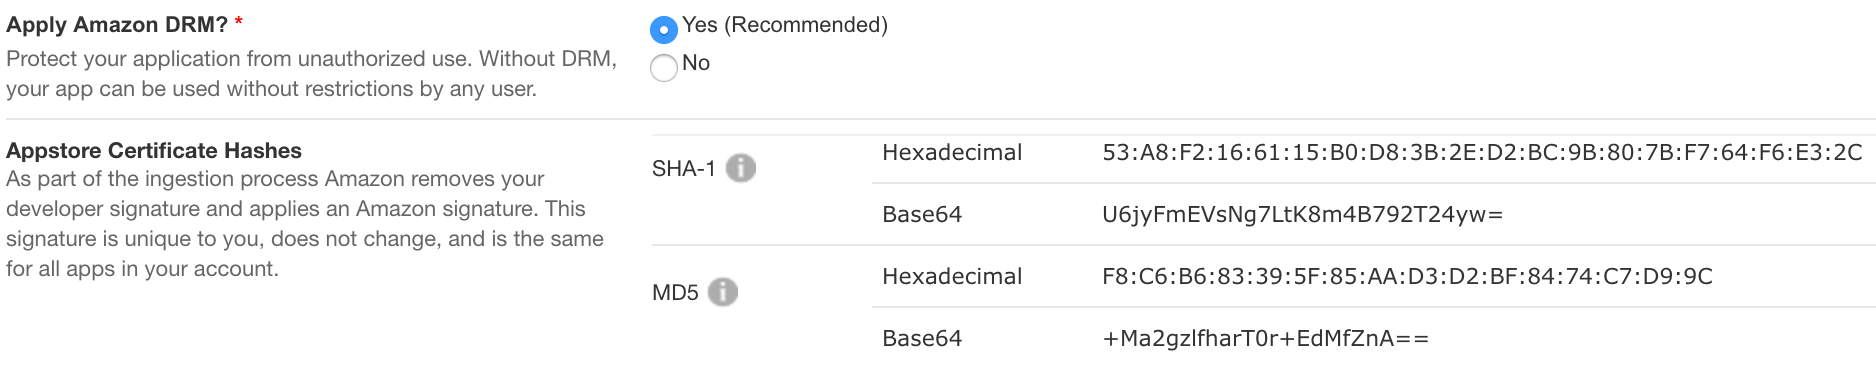
\includegraphics[width=1\textwidth]{data/amazon.png}
    \caption{Developer preferences in the Amazon developer console \cite{amazonDeveloper}}
    \label{fig:amazon}
\end{figure}

\begin{figure}[h]
    \centering
    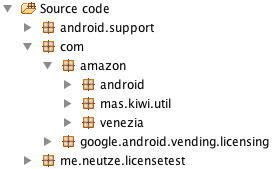
\includegraphics[width=0.3\textwidth]{data/amazonFolder.png}
    \caption{Amazon library structure in decompiled application}
    \label{fig:amazonFolder}
\end{figure}

%
different approach to perform license verification and enforce result
google lvl include and integrate modified version of lvl library, not required to implement any mechanism on their own, done by amazon packaging tool
when submitting can check amazon DRM (see picture), applay amazon DRm to "Protect your application from unauthorized use. Without DRM, your app can be used without restrictions by any user." as the description says
"As part of the ingestion process Amazon removes your developer signature and applies an Amazon signature. This signature is unique to you, does not change, and is the same for all apps in your account."  as the description says, so developer signing the application by the develoepr before submitting is not necessary, amazon decompiles apk, injects drm code, compiles it and signs it with the "amazon developer" certificate
\cite{munteanLicense}
%

amazon appstore has to be installed the whole time and user has to be logged in order that the DRM works
